% Chapter Template

\chapter{Implementació} % Main chapter title

\label{Implementacio} % Change X to a consecutive number; for referencing this chapter elsewhere, use \ref{ChapterX}

En aquest apartat s'explica de quina manera s'han utilitzat les tecnologies seleccionades per al desenvolupament.

\begin{itemize}
\item{}\textbf{Inici de sessió}\\

Per a l'inici de sessió s'utilitza el servei que proporciona \textit{Google}. L'aplicació mostra a l'usuari el botó d'inici de sessió d'aquesta plataforma, quan es prem aquest botó es desvia l'inici de sessió a \textit{Google} (figura 9.1) on l'usuari introdueix les dades del seu compte.

\begin{figure}[!h]
\centering
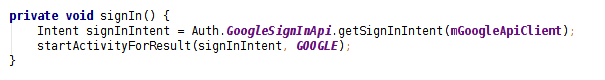
\includegraphics[scale=0.9]{Figures/initSessio1.png}
\caption{Crida d'inici de sessió}
\end{figure}

Un cop l'usuari ha introduit les seves dades a \textit{Google} es retorna el control al sistema. Quan l'aplicació continua amb la seva execució ho fa a partir de la funció que es pot veure en la figura 9.2. L'últim pas per a l'inici de sessió es obtenir les dades de l'usuari i iniciar l'aplicació.

\begin{figure}[!h]
\centering
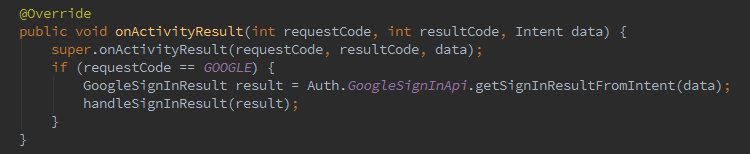
\includegraphics[scale=0.8]{Figures/initSessio2.png}
\caption{Retorn d'inici de sessió}
\end{figure}

\item{\textbf{Accés a la base de dades}}\\

La connexió amb la base de dades es dur a terme des de la classe \textit{FirebaseRepository}, aquesta classe és la classe genèrica que utilitzarant tots els serveis per tal d'accedir a la base de dades. En la figura 9.3 es pot veure com s'inicialitzen els camps del repositori.

\clearpage

\begin{figure}[!h]
\centering
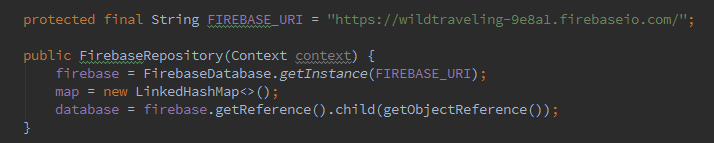
\includegraphics[scale=0.8]{Figures/db1.png}
\caption{Constructor del repositori}
\end{figure}

Dins d'aquesta classe es defineixen totes les operacions que es poden fer sobre la base de dades. En la figura 9.4 es pot veure com es declara un \textit{insert}.

\begin{figure}[!h]
\centering
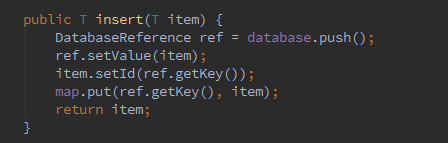
\includegraphics[scale=0.8]{Figures/db2.png}
\caption{Funció d'\textit{insert} genèrica}
\end{figure}

Per tal de llegir dades de firebase, el que es fa és el següent. Quan s'inicia l'aplicació es carreguen totes les dades de l'usuari en els repositoris. A més, per tal de tenir sempre els repositoris actualitzats, s'implementen \textit{listeners}. Quan es carreguen les dades provinents de \textit{Firebase} a les estructures del sistema es necessita convertir les dades del núvol en objectes del sistema. Per aquest motiu, s'utilitza la funció convert que es pot veure en la figura 9.5.

\begin{figure}[!h]
\centering
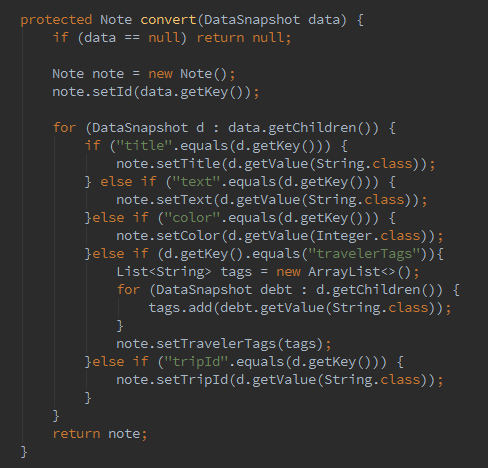
\includegraphics[scale=0.8]{Figures/db3.png}
\caption{Conversió de les dades a l'entitat Nota}
\end{figure}

\item{\textbf{Accés a les dades des de l'\textit{Activity}}}\\

Per interaccionar amb les dades i poder mostrar-les a l'usuari s'implementen diversos serveis. Aquests serveis són els encarregats de fer les operacions necessaries per tal de proporcionar a l'\textit{Activity} les dades que vol mostrar a l'usuari o per tal d'emmagatzemar les dades que l'usuari introdueix.\\

Es declara un servei per cada funcionalitat: un servei pels diferents tipus de persones, un per als viatges, un per despeses i deutes, i un altre per a les notes. En cada servei tenim una instància de repositori del tipus que estem tractant, per exemple, en el servei que tracta les despeses tenim una instància del repositori de despeses i una instància del repositori de deutes. En el servei es defineixen operacions com la de la figura 9.6.


\begin{figure}[!h]
\centering
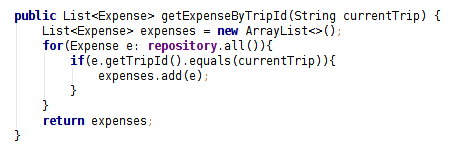
\includegraphics[scale=0.8]{Figures/serv1.png}
\caption{Mètode de la classe ExpenseService}
\end{figure}

Pel que fa a l'\textit{Activity}, es declara el servei com en la figura 9.7 i s'utilitza aquest servei per tal d'obtenir qualsevol dada i guardar les dades introduides per l'usuari.

\begin{figure}[!h]
\centering
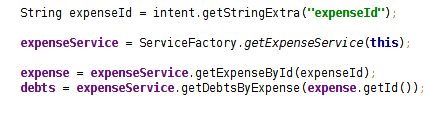
\includegraphics[scale=0.8]{Figures/serv2.png}
\caption{Mètode de la classe ExpenseService}
\end{figure}

\item{\textbf{Connexió amb serveis externs}}\\

En la connexió amb els serveis externs que s'utiltizen s'utilitza la mateixa arquitectura que en l'accés a les dades. Des del punt de vista de l'\textit{Activity}, el procediment és exactament el mateix. S'instància el servei que es necessita obtenint-lo de la factoria de serveis i s'utilitza per tal d'obtenir les dades que es necessiten.\\

La diferencia es veu en la classe servei, ja que enlloc de comunicar-se amb la base de dades es comunica amb un servei extern. En la figura 9.8 i 9.9 es pot veure un exemple de crida al servei extern que proporciona la llista dels hospitals que hi ha al voltant de l'usuari i posteriorment es selecciona el més proper a l'usuari. El resultat de la crida als diferents serveis sempre és un JSON el qual es deserialitza per tal d'obtenir objectes útils per al sistema.\\

\begin{figure}[!h]
\centering
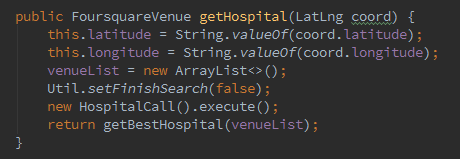
\includegraphics[scale=0.8]{Figures/api2.png}
\caption{Mètode per obtenir l'hospital més proper}
\end{figure}

\begin{figure}[!h]
\centering
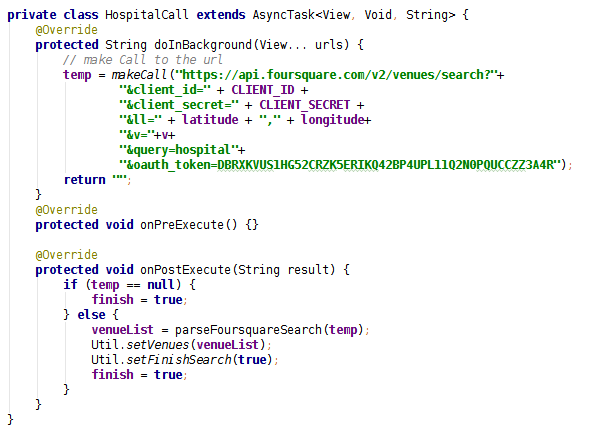
\includegraphics[scale=0.8]{Figures/api1.png}
\caption{Crida al servei de punts d'interés}
\end{figure}

\item{\textbf{Enviar correu electrònic}}\\

Per tal de poder enviar un correu electrònic directament des del codi \textit{Android} s'utilitza una classe anomenada MailSender. En aquesta classe es defineixen tots els paràmetres que permetran enviar un correu electrònic. En la figura 9.10 es pot veure el fragment de codi on es defineixen els paràmetre que permeten enviar des de \textit{Gmail}, s'inicia la sessió amb les credencials del compte \textit{WildTraveling} i es crea i envia el missatge en si.

\clearpage

\begin{figure}[!h]
\centering
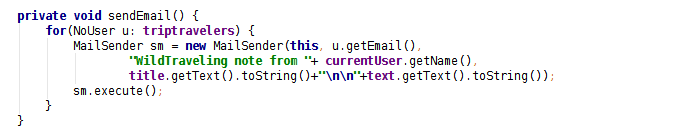
\includegraphics[scale=0.8]{Figures/email.png}
\caption{Enviament d'un correu electrònic}
\end{figure}

Des de l'\textit{Activity}, per tal d'enviar un email, es crea una instància de la classe MailSender amb les dades del receptor del correu, l'assumpte i el cos, i s'executa el procés que s'ha definit dins la classe (Figura 9.11).

\begin{figure}[!h]
\centering
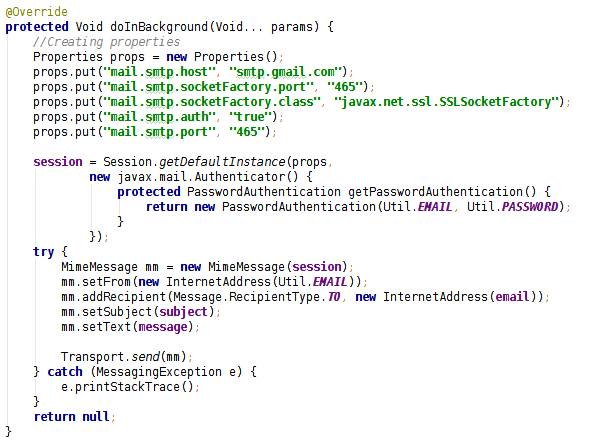
\includegraphics[scale=0.8]{Figures/email2.png}
\caption{Funció enviar correu electrònic}
\end{figure}

\end{itemize}